% arara: pdflatex
% arara: bibtex
% arara: pdflatex
% arara: pdflatex
% 
% Annual Cognitive Science Conference
% Sample LaTeX Paper -- Proceedings Format
% 

% Original : Ashwin Ram (ashwin@cc.gatech.edu)       04/01/1994
% Modified : Johanna Moore (jmoore@cs.pitt.edu)      03/17/1995
% Modified : David Noelle (noelle@ucsd.edu)          03/15/1996
% Modified : Pat Langley (langley@cs.stanford.edu)   01/26/1997
% Latex2e corrections by Ramin Charles Nakisa        01/28/1997 
% Modified : Tina Eliassi-Rad (eliassi@cs.wisc.edu)  01/31/1998
% Modified : Trisha Yannuzzi (trisha@ircs.upenn.edu) 12/28/1999 (in process)
% Modified : Mary Ellen Foster (M.E.Foster@ed.ac.uk) 12/11/2000
% Modified : Ken Forbus                              01/23/2004
% Modified : Eli M. Silk (esilk@pitt.edu)            05/24/2005
% Modified : Niels Taatgen (taatgen@cmu.edu)         10/24/2006
% Modified : David Noelle (dnoelle@ucmerced.edu)     11/19/2014

%% Change "letterpaper" in the following line to "a4paper" if you must.
 
\documentclass[10pt,letterpaper]{article}
 
\usepackage{hyperref}
\usepackage{cogsci}
\usepackage{pslatex}
\usepackage{amsfonts}
\usepackage{graphicx}
\usepackage{apacite}
\usepackage{color}
\usepackage{todonotes}
\usepackage{dsfont}
\usepackage{array}
\usepackage{textcomp}
\usepackage{multirow}

\definecolor{Red}{RGB}{255,0,0}
\newcommand{\red}[1]{\textcolor{Red}{#1}}

\newcommand{\jd}[1]{\green{$^*$}\marginpar{\footnotesize{JD: \green{#1}}}}
\definecolor{Green}{RGB}{10,200,100}
\newcommand{\ndg}[1]{\textcolor{Green}{[ndg: #1]}}


\newcommand{\subsubsubsection}[1]{{\em #1}}
\newcommand{\eref}[1]{(\ref{#1})}
\newcommand{\tableref}[1]{Table \ref{#1}}
\newcommand{\figref}[1]{Figure \ref{#1}}
\newcommand{\appref}[1]{Appendix \ref{#1}}
\newcommand{\sectionref}[1]{Section \ref{#1}}

\title{Pragmatics account for apparent limits on theory of mind use in adults}
 
\author{{\large \bf Robert X.~D.~Hawkins, Noah D.~Goodman}\\
  \{rxdh,ngoodman\}@stanford.edu\\
  Department of Psychology, 450 Serra Mall \\
  Stanford, CA 94305 USA}


\begin{document}

\maketitle

\begin{abstract}
?

\textbf{Keywords:} 
?
\end{abstract}

\section{Introduction}
\label{sec:intro}

\begin{figure*}[t!]
\begin{center}
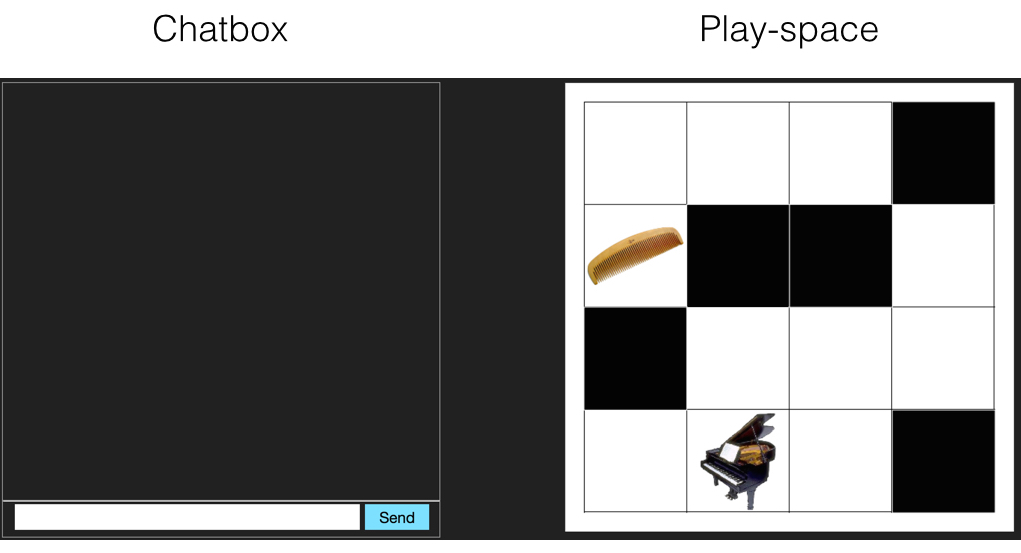
\includegraphics[scale = .35]{images/overall_view.jpg}
\end{center}
\vspace{-.25cm}
\caption{Interface used in the reported experiments. Objects behind the black squares were hidden from the director. \todo[inline]{TODO: Use images from tape condition, add extra panel to show matcher view.}}
\label{fig:interface}
\end{figure*}

Humans can accurately and intelligently reason about the mental states of other humans. Among other things, this ability -- called \emph{theory of mind} \cite{PremackWoodruff78_ChimpanzeeToM} -- allows us to infer the underlying beliefs and intentions that motivate others' actions, and to use these inferences to predict future actions \cite{BakerSaxeTenenbaum09_ActionUnderstandingInversePlanning}. Children acquire this ability by at least age six \cite{WimmerPerner83_BeliefsAboutBeliefs, WellmanCrossWatson01_ToMMetaAnalysis} and it serves as an important landmark in the developmental trajectory of intuitive theory use \cite{GopnikWellman12_ReconstructingConstructivism}.
%
While theory of mind use often appears to be automatic and effortless, Keysar and colleagues \cite{KeysarBarr___Brauner00_TakingPerspective, KeysarLinBarr03_LimitsOnTheoryOfMindUse, LinKeysarEpley10_ReflexivelyMindblind} have argued that it is actually the opposite, even for adults: we are ``mindblind" by default and only overcome our egocentric biases through an effortful process of perspective-taking. In other words, while adults are \emph{capable} of applying theory of mind reasoning, we do not always apply it reliably. 

In this paper we argue that the apparent failures this view is based on are in fact successes for sophisticated social reasoning. 
In particular, we argue that critical utterances used by Keysar and colleagues are \emph{uncooperative}: they are less informative than what a speaker would actually produce in that situation; listeners expect these more informative utterances, and interpret the actual utterances accordingly---resulting in ``errors''.

The argument of Keysar and colleagues is based on an elegant experimental paradigm, where participants played a simple communication game with a confederate. The two players were placed on opposite sides of a $4 \times 4$ grid containing a set of everyday objects.
\todo[inline]{Refer to updated Fig.~1 with both director screen and matcher screen }
The confederate played the role of `director,' giving instructions about how to move objects around a grid, and the participant played the role of `matcher,' attempting to follow these instructions. For example, the objects in one trial included a medium-sized measuring cup in one location and a smaller measuring cup in another location. The director gave an instruction like `move the large cup up one square,' referring to the medium-sized one. 
Some objects were occluded such that only the matcher could see them, creating an asymmetry in the players' knowledge. To perform accurately on critical trials, the matcher would need to apply theory of mind to reason about the director's beliefs. For example, imagine a much larger measuring cup were placed in an occluded slot: if a participant failed to account for the director's (partial) knowledge, she might interpret `the large cup' to mean this occluded cup (which the director couldn't possibly know about). 
Indeed, \citeA{KeysarLinBarr03_LimitsOnTheoryOfMindUse} found that participants attempted to move the hidden item in 30\% of cases: 71\% of participants attempted to move this hidden item at least once (out of four critical cases) in the experimental condition, compared to 0\% in a control condition where there was no ambiguity over the referent. 
%46\% of participants reached for the hidden object at least twice. 
Additionally, eye-tracking data showed that participants considered the hidden item more often and for longer in the experimental condition than the control condition. 

While these results are compelling, the paradigm has been criticized from several different angles. First, in all experiments, the privileged object was a better fit for the referring expression than the one in common ground (e.g. the largest measuring cup vs. the medium measuring cup for ``the large measuring cup"), making the privileged object \emph{a priori} more likely to be the referent. It would be fairer to compare two objects that fit the referring expression equally well \cite{HellerGrodnerTanenhaus08_Perspective}. Second, the viewpoint asymmetry paradigm is somewhat unnatural: common ground is typically built incrementally over the course of an interaction rather than presented all at once, and it is rare for a shared display to differ in perceptual accessibility \cite{HannaTanenhausTrueswell03_CommonGroundPerspective}. Third, none of the experiments reported by Keysar and colleagues included a key comparison condition where the critical item (e.g. the largest measuring cup) was \emph{also} in common ground \cite{BrownSchmidtHanna11_IncrementalPerspectiveTaking}---perhaps people would refer to the critical item less in the privileged condition than in the full common ground condition, which would put a more positive spin on the results. %Note that none of these criticisms invalidate the paradoxical result that listeners move an occluded object, they just suggest an alternative explanation. Reference disambiguation is probabilistic: common ground and goodness of fit are weighed against one another.

In this paper, we offer an additional factor that helps account for Keysar's results. 
Theory of mind as applied within language understanding depends on an accurate model of what a speaker would say in different situations; given an utterance, a listener can then reason backward to the most plausible situation.
This suggests that we consider whether the utterances used by the confederate in Keysar's critical conditions were actually what a speaker would be expected to say. 
If not, then perhaps participants are making choices that are in fact consistent with correct pragmatic interpretation on the confederate's (uncooperative) utterance.
More precisely, when both players know that objects are occluded in the display, the speaker may tend to add additional precision to references in order to avoid confusion. If the listener \emph{expects} the speaker to do this, they will pragmatically pick the \emph{a priori} more likely referent of the referring expression, which in critical trials will be the occluded object. In other words, it is precisely \emph{because} the listener takes the speaker's mental state into consideration that they are tricked by an uncooperative confederate into choosing the wrong item. 
%=======
%Some objects were occluded such that only the matcher could see them, creating an asymmetry in the players' knowledge. To perform accurately, the matcher would need to apply theory of mind and reason about the director's beliefs. For example, if a much larger measuring cup were placed in an occluded slot and agents failed to account for the director's beliefs, they might interpret `the large cup' to mean this occluded cup even though the director couldn't possibly know about it. Indeed, \citeA{KeysarLinBarr03_LimitsOnTheoryOfMindUse} found that participants attempted to move the hidden item in 30\% of cases: 71\% of participants attempted to move this hidden item at least once (out of four critical cases) in the experimental condition, compared to 0\% in a control condition where there was no ambiguity over the referent. 46\% of participants reached for the hidden object at least twice. Additionally, eye-tracking data showed that participants considered the hidden item more often and for longer in the experimental condition than the control condition. 
%>>>>>>> 179ee1de2933b596af109cc10f157c31fdcea761

We began by replicating \citeA{KeysarLinBarr03_LimitsOnTheoryOfMindUse} in a multi-player web experiment. We recruited participants to be both director and matcher (instead of using a confederate), but instructions for critical items, as well as a random subset of filler items, remained scripted as in the original study. We replicated the original finding, but noted a tendency of directors to be ove-rinformative in unscripted trials. We then ran the same experiment without scripting the directions for critical trials, observing unconstrained director behavior. We observe much greater precision in unconstrained director utterances and better performance of the matchers. This minimal pair of experiments demonstrates that listener mistakes are at least partially due to the pragmatics of the task, ironically showing that apparent failures of theory of mind are in fact attributable to sophisticated expectatuions about speaker behavior---that is, to theory of mind.

\ndg{intro can probably be compressed some if needed.}

\begin{table*}
\begin{center}
\begin{tabular}{ p{2cm} | r | r |  r || r | r | r || r | r | r}
& \multicolumn{3}{c||}{\% attempted at least once} & \multicolumn{3}{c||}{\% attempted at least twice} & \multicolumn{3}{c}{\% of total cases}\\
\hline
& Orig. & Exp. 1 & Exp. 2 & Orig. & Exp. 1 & Exp. 2 & Orig. & Exp. 1 & Exp. 2  \\
Experimental & 71 & 93 & 61 & 46 & 57 & 32 & 30 & 43 & 24\\
Baseline        & 0   & 7   & 0   & 0   & 0   & 0   & 0   & 2   & 0\\
\end{tabular}
\caption{Side-by-side comparison of error rates in \citeA{KeysarLinBarr03_LimitsOnTheoryOfMindUse} and our two replications. The first section shows the percentage of \emph{participants} attempting to move the occluded distractor at least one of the four possible cases. The second section shows the percentage attempting to move it at least twice. The third section shows the percentage of \emph{all experimental trials} that the participant actually tried to move the occluded object. \todo[inline]{Big caption maybe unnecessary. Anything else to include in this table? Maybe Keysar et al, 2000, which reported \% of total cases, or our Exp. 2 results if you remove the two most difficult items? There, errors drop quite a lot.}}
\label{table:mainResults}
\end{center}
\end{table*}

\section{Exp.~1: Scripted Replication}
\label{sec:Exp1}

\subsection{Participants}

We recruited 34 participants (17 pairs) from Amazon Mechanical Turk. All participants were from the U.S. Three pairs were excluded for making 2 or more errors on non-critical items.

\subsection{Materials \& Procedures}


Participants interacted in a real-time, multi-player environment on the web \cite{Hawkins15_RealTimeWebExperiments}. 
%To deal with participants arriving at unpredictable times, we implemented a waiting room mechanism, where the first person to enter the game environment would see a screen saying ``Waiting for another player..." and the second person would trigger the game to start. 
Pairs of participants---assigned randomly to `director' and `matcher' roles---interacted with one another through a web interface, shown in Fig. \ref{fig:interface}. On the left side of the screen, participants could freely type messages to one another; on the right side the screen, players could view a set of objects placed in a 4 x 4 grid. Five of the grid cells were occluded from only the director's perspective, and the remaining 11 were visible to both matcher and director. Six or seven objects were displayed in the grid at a given time. One of these objects was a `target', such as a cassette tape, placed in an unoccluded cell such that both participants could see it. Another object, such as a roll of tape, was placed in an occluded slot such that it was only visible to the matcher. The rest of the objects were unrelated `fillers' placed in random locations. We used the same set of targets and occluded alternatives as \citeA{KeysarLinBarr03_LimitsOnTheoryOfMindUse}, but we were unable to obtain the filler objects from the original experiment and created our own.
Before entering the game environment, every participant independently passed a short quiz about the task's instructions, ensuring that they understood the interface. Among other items on the quiz, we verified that both participants understood that items behind black cells were only visible to the matcher. 

The experiment was composed of eight items, with each item using a different set of objects. Each item included one `critical pair' of objects, one of them the target and the other hidden, such as the cassette tape and the roll of tape. For each item, we gave the director a series of four instructions to move objects around, which were displayed as a series of arrows pointing from some object to an unoccupied cell. 
To collect clean mouse-tracking data, we began every instruction by asking the matcher to click a small circle in the center of the grid. After this small circle was clicked, the director was allowed to communicate the next instruction and we started recording from the matcher's mouse. 
One of the instructions was a `critical instruction,' which referred to the target object.
For half the instructions, directors were free to communicate however they wished. For the other half, including all the critical instructions, their messages to the matcher were pre-scripted such that we could use the precise wording from \citeA{KeysarLinBarr03_LimitsOnTheoryOfMindUse}. For example, when giving instructions on how to move the cassette tape, the director would be forced to use the ambiguous utterance ``Move the tape down one square." (That is, in these conditions, the scripted message would automatically appear in the director's chat window, and they would have to click `send' for the experiment to continue.)

We collected baseline performance for each condition by replacing the hidden alternative (e.g.~a roll of tape) with an object that did not fit the critical instruction (e.g.~a battery); we used the same unambiguous replacements as \citeA{KeysarLinBarr03_LimitsOnTheoryOfMindUse}. Each participant received half the items in the experimental condition and half in the baseline condition. The assignment of items to conditions was randomized across participants, and the order of conditions was randomized under the constraint that the same condition would not be used on more than two consecutive items. All object sets, object placements, and corresponding instruction sets were the same for all participants.

This paradigm differs from those used by \citeA{KeysarLinBarr03_LimitsOnTheoryOfMindUse} in three primary ways. First, participants were not seated across from each other at a table: they each saw a views of the 4 x 4 grid on screen and communicated via a text box. Second, we did not use a trained confederate. We randomly assigned one of the players to the role of the instruction giver, and maintained the original wording by scripting a subset of their instructions. Finally, the hidden object was not placed in a bag, in which respect our design more closely resembles \citeA{KeysarBarr___Brauner00_TakingPerspective}.

%The experiment proceeded through all eight items, with the director providing instructions and the participant moving the objects. Except for instructions with scripted messages, the participants were free to use the chat box for questions, small talk, or whatever else.
\begin{table*}
\begin{center}
\begin{tabular}{ m{.75cm} | m{1.5cm} | m{1.5cm} | m{1.5cm} |  m{1.25cm} | m{1.6cm} | m{1.4cm} | m{1.3cm} | m{1.3cm} | m{1.5cm} |}
& & Item 1 & Item 2 & Item 3 & Item 4 & Item 5 & Item 6 & Item 7 & Item 8\\\hline
& instruction & ``glasses'' & ``bottom block'' & ``tape'' & ``large measuring cup'' & ``brush'' & ``eraser'' & ``small candle'' & ``mouse'' \\\hline
& target & sunglasses & block (3rd row) & cassette & medium cup & round hairbrush & board eraser & medium candle & computer mouse \\\hline
& hidden distractor & glasses case & block (4th row) & scotch-tape & large cup & flat \,\,\,hairbrush & pencil eraser & small candle & toy mouse \\
 \hline\hline
\multirow{2}{.75cm}{Exp.~1}  & \# incorrect & 0 & 5 & 1 & 3 & 2 &6 & 6 & 1 \\ 
                                               & \# correct & 6 & 3 & 1 & 8 & 2 & 2 & 4 & 6 \\
 \hline\hline
\multirow{2}{.75cm}{Exp.~2} & \# incorrect & 0 & 1 & 1 & 3 & 9 & 7 & 1 & 5 \\
                                              & \# correct   & 12&14&11&13&7 &8   &12& 8 \\

\end{tabular}
\caption{Item-wise error rates}
\label{table:ItemWise}
\end{center}
\end{table*}


\subsection{Results and discussion}

In Table \ref{table:mainResults} we show the error rates on critical items, and compare to the data from
\citeA{KeysarLinBarr03_LimitsOnTheoryOfMindUse}.
We find that 93\% of participants (all but one) attempted to move the hidden distractor at least once in the Experimental condition, out of four possible items, compared to only 7\% (only one) in the baseline condition. This is similar to the effect observed by the authors in the original study, which found 71\% and 0\%. Our errors were larger across the board, perhaps due to the interface or the population, but the gap between the two conditions is roughly the same size.
%Next, we examine whether there are differences in error rates across items. 
In Table \ref{table:ItemWise}, we break down the pattern of errors by item. 
%Because our randomization procedure undersampled the experimental condition for several items, a chi-squared test is inappropriate. Using Fisher's exact test, we cannot reject the null hypothesis of independence ($p = 0.13$). Still, 
We note that several conditions have much higher error rates than others -- for example, 75\% of participants in the experimental condition of item 6 made an error (the ``whiteboard eraser'' vs. the ``pencil eraser'') while only 17\% of participants in item 8 made an error (the ``computer mouse'' vs. the ``toy mouse''). 
This suggests that the dependent variable highlighted in the original study (i.e. ``percentage of participants who moved the critical item at least once'') is somewhat problematic. It could look like 100\% of participants made errors even if they all made those errors on one particularly difficult item. Indeed, if we exclude the three `hard' items where over 60\% of participants in the experimental condition made errors, this dependent variable drops from 93\% to only 43\% of participants. 
%This suggests that the ``at least one error'' DV is not appropriate in settings with high variability across items and that we might want to be more careful about controlling for this variability, perhaps by first measuring salience and ambiguity without the occlusion aspect of the paradigm.

As a proxy for the eye-tracking analyses reported by \citeA{KeysarLinBarr03_LimitsOnTheoryOfMindUse}, we conducted a mouse-tracking analysis. We define the decision window as the span of time between the point when the matcher received their instruction message and when they started moving an object. If it took them multiple attempts to move the correct object, we restricted our analysis to the first attempt. We took the set of all mouse position samples in the decision window (collected approximately every 15ms), and measured what proportion were located inside the cell containing the target vs. the cell containing the distractor.  We had to exclude an additional 3 participants for this analysis, because the timestamps for director and matcher did not align and we could not establish the decision window properly.
We found that there is an interaction between cell type and condition on the percent of hover time spent in that cell, $b = -0.21, t(11) = -3.1, p = 0.003$. In baseline trials, people spent much more time in the target cell and much less time in the distractor cell than in the experimental condition (see Fig. \ref{fig:exp1hover}).\footnote{Note that this analysis includes participants who actually made errors, since the data is too sparse to exclude them.} %accounts for a significant proportion of variance $F(3, 52) = 10.7, p < 0.001$

By running this replication as a multi-player web experiment we have available an additional source of data beyond the original experiments: half of the instructions were unscripted, providing observations of natural production of referential descriptions for filler items. 
Informally, we noted a tendency toward, possibly unnecessary, precision in descriptions. Instead of ``move the stuffed animal down'', participants say ``move the stuffed panda bear down.'' Or, instead of saying ``move the plane to the right'' when there is only one plane, participants say ``move the red airplane to the right.'' 
Perhaps directors were taking the time to make more precise descriptions because they believed it was contextually relevant: both parties know that there are hidden objects in the environment increasing the chance of miscommunication from imprecise descriptions. 
If the matcher expected the director to be precise, then they would be justified in picking the first or best object that meets the description (rather than worrying excessively about occluded cells). 
That is, the scripted instructions used by the director for critical trials may have been \emph{uncooperative}, and thus led matchers astray. 
We tested this prediction in Exp.~2, where we removed the scripted instructions and allowed speakers to refer to items however they wished.
By the reasoning above we expect to see more precise descriptions by unscripted directors and fewer errors by matchers in the critical trials.


%\subsection{Discussion}
%
%In both raw patterns of error and mouse-tracking metrics, we successfully replicated the findings of \citeA{KeysarLinBarr03_LimitsOnTheoryOfMindUse}. Participants frequently attempted to move the occluded alternative when it matched the target referential expression, even though the director couldn't possibly have been referring to it. Furthermore, the matcher tended to spend more time hovering their cursor over the occluded cell, and less time hovering over the target object, in ambiguous experimental trials than in baseline trials with no ambiguity. Both of these results support Keysar's claim that adults do not reliably deploy theory of mind reasoning when it is called for.
%
%Still, in running this replication as a multi-player web experiment, we observed two particularly interesting features in the data. First, 
%
%our analysis of item-level differences shows that the dependent variable highlighted in the original study (i.e. ``percentage of participants who moved the critical item at least once'') is somewhat problematic. It could look like 100\% of participants made errors even if they all made those errors on one particularly difficult item. Indeed, if we exclude the three `hard' items where over 60\% of participants in the experimental condition made errors, this dependent variable drops from 93\% to only 43\% of participants. This suggests that the ``at least one error'' DV is not appropriate in settings with high variability across items and that we might want to be more careful about controlling for this variability, perhaps by first measuring salience and ambiguity without the occlusion aspect of the paradigm.

%Second, because half of the instructions were unscripted, we were able to observe natural production of referential descriptions for a number of fillers. Informally, we noted a tendency toward over-informativity. Instead of ``move the stuffed animal down'', they'll say ``move the stuffed pa'nda bear down.'' Or, instead of saying ``move the plane to the right,'' they'll say ``move the red airplane to the right,'' even though there is only one plane. This suggested that the confederate's scripted instructions were in some sense uncooperative and counter to the matcher's expectations. Perhaps directors were taking the time to make more costly over-informative descriptions because they believed it was contextually relevant: both parties know that there are hidden objects in the environment. If the matcher reasoned in this way and expected the director to be overinformative, then they would be justified in picking the first object that meets the description rather than worrying about occluded cells. We tested this prediction in Exp.~2, where we removed the scripted instructions and allowed speakers to refer to items however they wished. If speakers really are being overinformative, and listeners are correctly expecting this, we should see fewer errors after removing uncooperative scripts.

\section{Exp.~2: Unscripted Replication}
\label{sec:Exp2}

\subsection{Participants}

We recruited 64 participants (32 pairs) from Amazon Mechanical Turk, roughly doubling the sample size from Exp.~1. All participants were from the U.S. Three participants were excluded for making 2 or more errors on non-critical items, and one additional participant was excluded because they were not a native English speaker.

\subsection{Materials \& Procedures}

Everything was the same as Exp.~1, except we did not use scripted messages for critical instructions. 
 
\subsection{Results}

Error rates are reported in Table \ref{table:mainResults}, alongside the results from \citeA{KeysarLinBarr03_LimitsOnTheoryOfMindUse} and our scripted replication in Exp.~1. Participants never moved the hidden object in the baseline condition, and total error rates for experimental trials are significantly lower than the rates found in Exp.~1, $\chi^2(1) = 5.35, p = 0.02$.

More dramatically, we find that patterns of errors in Exp.~2 diverge significantly from a uniform distribution across items, $\chi^2(7) = 24.8, p < 0.001$. Looking more closely at these patterns, we see that the only items where errors are consistently made are those where the costly over-informative utterance remains ambiguous. For example, in item 5, both the target and distractor are hair brushes: one is round and one is flat. ``Hair brush'' is already a label at the sub-class level. If we remove the two most difficult items (the ``hair brushes'' and the ``erasers''), the total percentage of errors on experimental trials drops from 26\% to 10\% and the percentage of participants making at least one error drops from 60\% to 32\%.

When we conducted a mouse-tracking analysis identical to the one reported for Exp.~1, we again found a significant interaction between condition and cell type on hover time, $b = -0.18, t(108) = -5.2, p < 0.001$. However, the effect is attenuated: in experimental trials, participants spend significantly more time hovering over the target than the distractor (see Figure \ref{fig:exp2hover}) whereas in Exp.~1, participants spent roughly the same amount of time hovering over each.

\todo[inline]{rdh: I don't think we have enough power to show a difference between mean hover-times in the two experiments -- the first experiment just didn't have a big enough sample (the psych254 class budget was a pretty hard constraint). Might be able to get more power by doing mixed model like below, or by calculating the times more precisely (currently, just count number of mouse movement events in time window, which probably adds a lot of noise).}

Next, we test whether these reductions in error rate and hover-time interference are in fact due to different speaker behavior. Two coders were given the list of messages that directors sent to convey instructions for critical items, blind to condition. The coders determined (1) whether or not the label used by the speaker fit the hidden distractor and (2) whether or not the label used by the director was more or less precise than the scripted label used in Exp.~1. Inter-rater reliability was relatively high, with Cohen's $\kappa=0.82$ for distractor fit and $\kappa=0.67$ for the precision comparison. Binary rater decisions were averaged to form a single distractor fit score for each message, and a single precision score.

We found that the referring expressions speakers used to convey critical instructions only fit the distractor 53\% of the time, compared to the scripted message in Exp.~1, which (by definition) fit the distractor 100\% of the time. 
\todo[inline]{Except that `glasses' one, which doesn't really apply to a glasses case. I'm now pretty sure that this is the fault of the picture I picked (an \emph{open} glasses case rather than a closed one\dots which was dumb in retrospect) Maybe I should re-run analyses without that item, just in case?} 
Furthermore, 47\% of these referring expressions were rated to be more precise than the corresponding scripted instruction used in Exp.~1. \ndg{was remaining 53\% rated as scripted more precise or mostly `can't tell'?} As expected, there's a strong negative relationship between the precision of the label and whether it might apply to the hidden distractor, $r = -0.73$. Finally, we used a mixed effects logistic regression model to estimate the effect of distractor fit and precision on the probability of making an error on critical trials. We included random intercepts for the eight items. We find that participants are significantly more likely to make an error when the label applies to the distractor, $b = 3.15, z = 2.93, p = 0.003$, but that precision has no effect, $p = 0.96$. 



\begin{figure}[b!]
\begin{center}
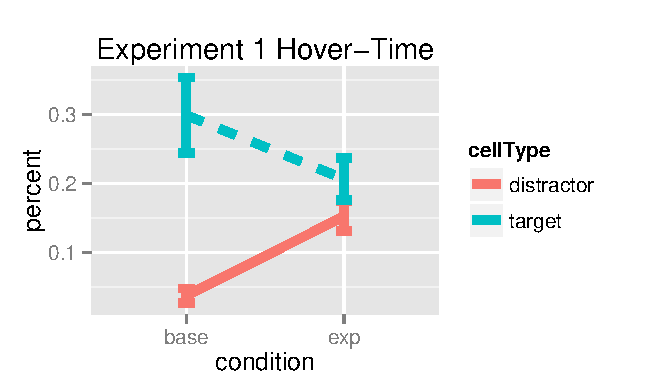
\includegraphics[scale=.75]{images/exp1MouseTracking.pdf}
\caption{Mean percentage of time spent hovering over the distractor and target cells in the experimental and baseline conditions. Error bars are 95\% confidence intervals.}
\label{fig:exp1hover}
\end{center}
\end{figure}

\begin{figure}[b!]
\begin{center}
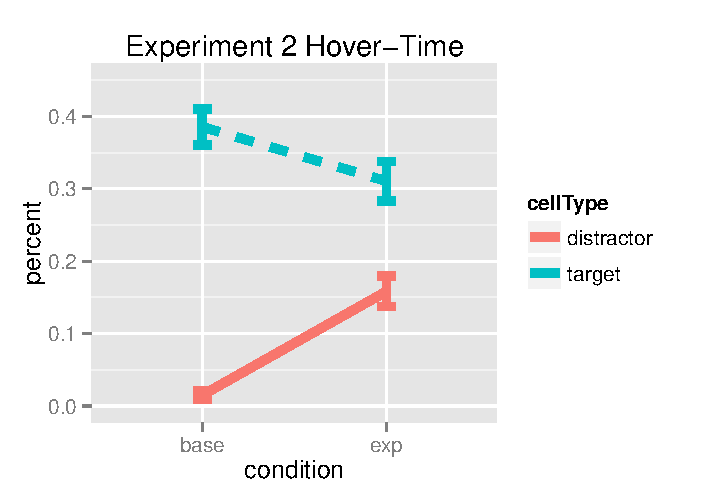
\includegraphics[scale=.75]{images/exp2MouseTracking.pdf}
\caption{Mean percentage of time spent hovering over the distractor and target cells in the experimental and baseline conditions. Error bars are 95\% confidence intervals.}
\label{fig:exp2hover}
\end{center}
\end{figure}

%\begin{itemize}
%\item people still try to move occluded objects, but they do it less, and that behavior is more confined to a few particularly difficult items.
%\item this happens because the scripted instructions we forced directors to use in Exp.~1 were unnatural and violated listener expectations of overinformativity
%\item the fact that the effect is attenuated in exp. 2 is actually evidence of some theory of mind use (insofar as the director choosing to be overinformative, and the matcher expecting overinformativity constitutes ToM
%\end{itemize}

\section{General Discussion}

Removing constraints on the speaker produced a dramatic reduction in overall matcher errors and systematic variation in error rates across items. How did unscripted speaker behavior differ from scripted behavior such that these effects emerged? We found that unscripted speakers systematically tended to produce more precise, costly referring expressions than their scripted counterparts -- for example, ``the clear audiocassette'' when there was only one ``tape'' in the speaker's display. These precise labels were less likely to fit the hidden distractor, and therefore less likely to lead to a matcher error.

A key point 

We noticed several differences between our study and \citeA{KeysarLinBarr03_LimitsOnTheoryOfMindUse} that prevented a direct replication. The primary difference between our study and the original is the fact that it will be run online with participants connected via a virtual environment, instead of face-to-face in a room. A related difference is our decision not to use a confederate. In general, studies using confederates are difficult to replicate exactly and are impractical to run online. We are aware that this change (while keeping scripted instructions, which were the primary justification for the confederate) may lead to additional variation across groups. It is also known that textual communication (via our instant messaging interface) can differ from verbal communication (as in the original study). Finally, the way people attempt to move things in our virtual environment may be different from how people attempt to move things in the lab, and we cannot eye-tracking data to back up our analysis, as the original paper did.

% Second, it's worth thinking about some ways our online version may differ from the original. The fact that we didn't use a confederate didn't seem to be a problem, given our use of randomly scripted instructions. Similarly, because players could type messages directly to one another, and since the director could watch the matcher moving objects in real-time, it's also fair to say that participants truly believed they were playing with another human being. 

\ndg{mention overinformativity in refexp somewhere in here...}

One major concern is our graphical representation of occluded cells. We told players that items behind black cells were hidden to the director, showed them side-by-side displays of the director and matcher views, and quizzed them on this detail in the short attention check that players had to pass before playing. But they may have forgotten part-way through the experiment, or failed to fully internalize it. In the in-lab version, there was an actual divider between players, so it would have been more salient. We suspect that some subset of errors in our version game aren't due to a failure of perspective-taking, but instead because of a misunderstanding of what the other person's perspective is to begin with. For example, one matcher wrote, ``This seems to work wether [sic] the space is black or not.'' This suggests that they thought that the black squares were obstacles or invalid destinations. However, this source of errors is held constant across our two experiments, and it would only bias our estimates of errors toward supporting Keysar's results, making our analysis conservative.

At a methodological level, the pair of experiments we report is a reminder that manipulations administered by a trained confederate can interact in unexpected ways with a participant's social and communicative expectations. Regardless of the experimental context, it's illuminating to see how real participants naturally interact, and 

\todo[inline]{rdh: methodological note that running multi-player control w/o confederate is important to know whether confederate behavior is valid and cooperative}


\section{Acknowledgements}

\small We're grateful to Boaz Keysar for providing select materials for our replication. Exp.~1 was originally conducted under the supervision of Michael Frank, with early input from Desmond Ong. This work was supported by ONR grants N00014-13-1-0788 and N00014-13-1-0287,  and a James S. McDonnell Foundation Scholar Award to NDG. RXDH was supported by the Stanford Graduate Fellowship and the National Science Foundation Graduate Research Fellowship under Grant No. DGE-114747. 

\bibliographystyle{apacite}

\setlength{\bibleftmargin}{.125in}
\setlength{\bibindent}{-\bibleftmargin}

\bibliography{bibs}


\end{document}
